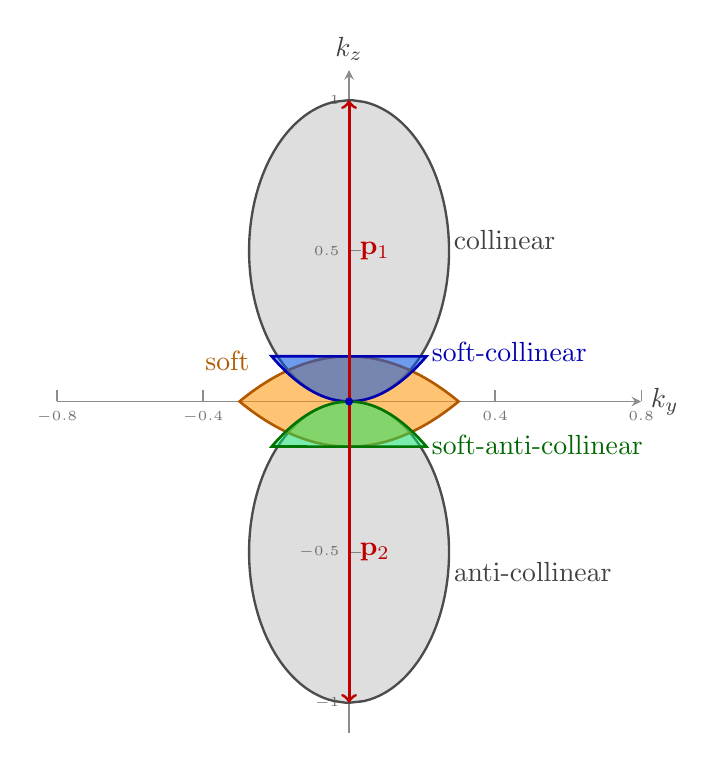
\begin{tikzpicture}
\begin{axis}[
  width=9cm,
  height=10cm,
  xmin=-0.8, xmax=0.8,
  ymin=-1.1, ymax=1.1,
  xtick distance=0.4,
  tick label style={black!55, font=\tiny},
  tick style={black!45, line width=0.45pt},
  axis lines=middle,
  axis line style={black!45, line width=0.55pt},
  xlabel={$k_y$},
  ylabel={$k_z$},
  xlabel style={anchor=west, text=black!75},
  ylabel style={anchor=south, text=black!75},
  tick align=inside,
  samples=160,
  clip=true,
]

% RegionPlot: y^2 + 0.3 z (1+z) < 0
% shifted upward by 1: plotted at vertical coordinate z+1
\path[
  fill=black!65,
  fill opacity=0.20,
  draw=black!70,
  line width=0.85pt
]
  plot[domain=-1:0, samples=180, variable=\z]
    (axis cs:{sqrt(-0.3*\z*(1+\z))},{\z+1})
  -- plot[domain=0:-1, samples=180, variable=\z]
    (axis cs:{-sqrt(-0.3*\z*(1+\z))},{\z+1})
  -- cycle;

\path[
  fill=black!65,
  fill opacity=0.20,
  draw=black!70,
  line width=0.85pt
]
  plot[domain=0:1, samples=180, variable=\z]
    (axis cs:{sqrt(0.3*\z*(1-\z))},{\z-1})
  -- plot[domain=1:0, samples=180, variable=\z]
    (axis cs:{-sqrt(0.3*\z*(1-\z))},{\z-1})
  -- cycle;

% softCollplot region 2
\path[
  fill=orange!85!yellow,
  fill opacity=0.55,
  draw=orange!70!black,
  line width=0.95pt
]
  plot[domain=-1.15:-1, samples=100, variable=\z]
    (axis cs:{sqrt(0.6*(\z+1.15))},{\z+1})
  -- plot[domain=-1:-0.85, samples=100, variable=\z]
    (axis cs:{sqrt(0.6*(-\z-0.85))},{\z+1})
  -- plot[domain=-0.85:-1, samples=100, variable=\z]
    (axis cs:{-sqrt(0.6*(-\z-0.85))},{\z+1})
  -- plot[domain=-1:-1.15, samples=100, variable=\z]
    (axis cs:{-sqrt(0.6*(\z+1.15))},{\z+1})
  -- cycle;

% softCollplot region 1
\path[
  fill=blue!65!cyan,
  fill opacity=0.50,
  draw=blue!70!black,
  line width=0.95pt
]
  plot[domain=-1:-0.85, samples=100, variable=\z]
    (axis cs:{sqrt(0.3*(\z+1))},{\z+1})
  -- plot[domain=-0.85:-1, samples=100, variable=\z]
    (axis cs:{-sqrt(0.3*(\z+1))},{\z+1})
  -- cycle;

% softCollplot2
\path[
  fill=green!55!cyan,
  fill opacity=0.45,
  draw=green!45!black,
  line width=0.95pt
]
  plot[domain=-0.15:0, samples=100, variable=\z]
    (axis cs:{sqrt(-0.3*\z)},{\z})
  -- plot[domain=0:-0.15, samples=100, variable=\z]
    (axis cs:{-sqrt(-0.3*\z)},{\z})
  -- cycle;

% Red arrows
\addplot[
  red!75!black,
  line width=1.1pt,
  ->
] coordinates {(0,0) (0,1)}
  node[midway, right, text=red!75!black] {$\mathbf{p}_1$};

\addplot[
  red!75!black,
  line width=1.1pt,
  ->
] coordinates {(0,0) (0,-1)}
  node[midway, right, text=red!75!black] {$\mathbf{p}_2$};

% Labels
\node[
  below right,
  text=orange!70!black
] at (axis cs:-0.42,0.2) {soft};

\node[
  below right,
  text=blue!70!black
] at (axis cs:0.2,0.23) {soft-collinear};

\node[
  below right,
  text=green!40!black
] at (axis cs:0.2,-0.08) {soft-anti-collinear};

\node[
  below right,
  text=black!75
] at (axis cs:0.26,0.6) {collinear};

\node[
  below right,
  text=black!75
] at (axis cs:0.26,-0.5) {anti-collinear};

% Origin marker
\addplot[
  only marks,
  mark=*,
  mark size=1.25pt,
  blue!70!black
] coordinates {(0,0)};

\end{axis}
\end{tikzpicture}


